\section{Vorwissen}
\vspace{-0.5cm}
\begin{minipage}{0.66\linewidth}
    Pythagoras-Bäume gehören zu den Fraktalen. Im zweidimensionalen Raum setzt sich ein Pythagoras-Baum aus 
    Quadraten zusammen, auf die jeweils ein rechtwinkliges Dreieck aufgesetzt werden, auf dessen Kanten
    wiederum Quadrate platziert werden.
    Sie tragen ihren Namen, da sich die Seitenlängen neuer Quadrate mittels dem Satz des Pythagoras 
    $a^2 + b^2 = c^2$ aus den Kantenlängen des aufgesetzten Dreiecks berechnen lassen.
\end{minipage}
\hfill
\begin{minipage}{0.3\linewidth}
    \centering
    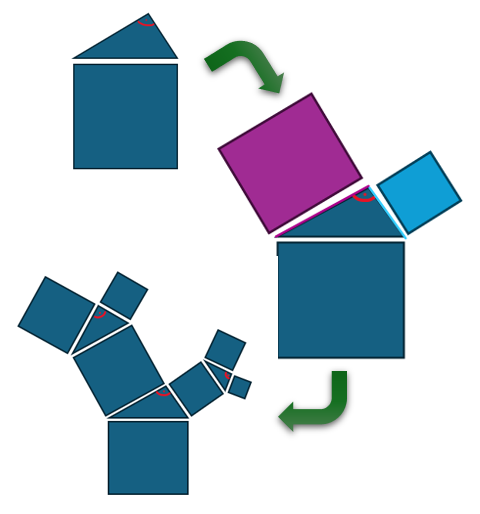
\includegraphics[width=\linewidth]{./pictures/Erzeugung-Pythagorasbaum.PNG}
    \captionof{figure}{Erzeugung eines Pythagoras-Baums}
    \label{fig:Erzeugung Baum}
\end{minipage}

\vspace{-0.5cm}
\subsection*{Mathematische Grundlagen}
\vspace{-0.25cm}
\subsubsection*{Kartesisches Koordinatensystem} \label{Koordinatensystem}
\vspace{-0.25cm}
\begin{minipage}{0.25\linewidth}
    \centering
    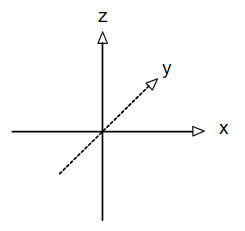
\includegraphics[width=0.8\linewidth]{./pictures/Koordinatensystem.PNG}
    \captionof{figure}{Achsenbeschriftung Koordinatensystem}
    \label{fig:koordinatensystem}
\end{minipage}
\hfill
\begin{minipage}{0.74\linewidth}
    Wir arbeiten mit einem dreidimensionalen Koordinatensystem, bei welchem die x-Achse bei frontaler 
    Betrachtung von links nach rechts verläuft, die y-Achse die Tiefe des Raums abbildet und die z-Achse 
    von unten nach oben verläuft.
\end{minipage}

\vspace{-0.25cm}
\subsubsection*{Bezeichner der Körper}\label{Koerper}
\vspace{-0.25cm}
\begin{minipage}{0.25\linewidth} % Würfel
    \centering
    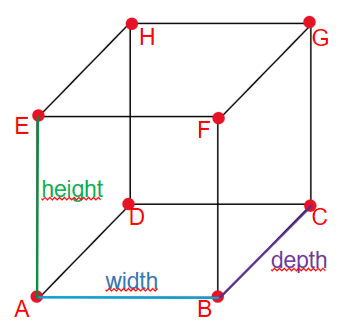
\includegraphics[width=\linewidth]{./pictures/Würfel.PNG}
    \captionof{figure}{Beschriftung Quader}
    \label{fig:wuerfel}
\end{minipage}
\hfill
\begin{minipage}{0.74\linewidth}
    Würfel / Quader\\
    Unsere Würfel und Quader sind definiert über die Ecken ABCD, welche das untere Quadrat bilden, und 
    die Ecken EFGH, welche das parallel darüberliegende Quadrat bilden.\\
    Darüber hinaus bestimmen die Seitenlängen width (entlang der x-Achse), depth (entlang der y-Achse) 
    und height (entlang der z-Achse) die Größe des Körpers.
\end{minipage}

\vspace{0.25cm} 
\noindent
\begin{minipage}{0.25\linewidth} % Dreieck
    \centering
    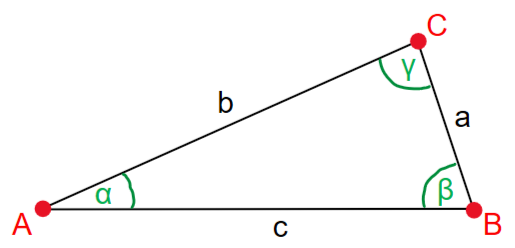
\includegraphics[width=\linewidth]{./pictures/Dreieck.PNG}
    \captionof{figure}{Beschriftung Dreieck}
    \label{fig:dreieck}
\end{minipage}
\hfill
\begin{minipage}{0.74\linewidth}
    Dreieck \\
    Dreiecke, die in unserem Programm für Dreiecksberechnungen wie den Sinussatz zum Einsatz kommen,
    folgen der in der Grafik dargestellten Beschriftung. Dabei ist $\gamma$ immer der rechte Winkel.
\end{minipage}

\subsubsection*{Betrag eines Vektors}\label{Vektorbetrag}
%\vspace{-0.25cm}
\[
\| \mathbf{v} \| = \sqrt{a^2 + b^2 + c^2}
\]

%\vspace{-0.25cm}
\subsubsection*{Sinussatz}\label{Sinussatz}
%\vspace{-0.25cm}\\
\[
\frac{a}{\sin(\alpha)} = \frac{b}{\sin(\beta)} = \frac{c}{\sin(\gamma)} \quad \Rightarrow \quad a = \frac{c}{\sin(\gamma)} \cdot \sin(\alpha),
\quad b = \frac{c}{\sin(\gamma)} \cdot \sin(\beta)
\]